\documentclass{article}
\usepackage[left=2cm, right=2cm, top=1cm]{geometry}
\usepackage[utf8]{inputenc}
\usepackage{amsthm,amsmath,amsfonts,amssymb,graphicx}
\usepackage{algorithm}
\usepackage{caption}
\usepackage{subcaption}
\usepackage[noend]{algpseudocode}

\title{Segmentation of heat-maps containing linear routes}
\author{\vspace{-10ex}}
\date{\vspace{-5ex}}

\begin{document}
\maketitle
\begin{abstract}
In this paper we present a heat-map segmentation algorithm. The proposed segmentation algorithm
segments a heat-map into high traffic regions and low traffic regions. The borders of the different regions often coincide with high traffic routes. We then test the proposed 
algorithm on a heat-map constructed from Automatic Identification System (AIS) data collected in the Celtic sea, the Channel and the Bay of Biscay. The results show that the approach shows promise and if improved further 
it could become a viable segmentation strategy.
\end{abstract}
Often, when we first inspect a dataset containing the temporal-spatial coordinates of multiple objects (i.e. the movements of say humans, animals or vessels)
we would create a heat-map (grid data onto a two-dimensional grid) so that we can build some intuition (gather information) about the data.
The information we extract from heat-maps (insight gained) can then be used to further analyze the original data. Some examples of the useful kind of information which can be extracted from a 
heat-map include: high traffic volume routes and regions. In this paper, we present an automatic heat-map segmentation algorithm which will allow us to automatically extract the 
 aforementioned pieces of information. In this paper we focus primarily on AIS data (shipping data). 
 
The pseudo-code of the proposed segmentation algorithm is given in Algorithm 1. 
\begin{algorithm}
 \caption{Polygon Heat-map Segmentation Algorithm}\label{euclid}
 \begin{algorithmic}[1]
 \Procedure{polygonSegmentation}{heatmap,coastlinemask,landmask}
 \State $\textrm{heatmap} \gets \log(\textrm{heatmap}+1)$
 \Comment{emphasizes the linear tracks}
 \State $\textrm{copy} \gets \textrm{heatmap}$
 \Comment{store a copy of original}
 \State $\textrm{heatmap} \gets \textrm{maskCoastline(heatmap,coastlinemask)}$
 \Comment{mask coastline}
 \State $\textrm{heatmap} \gets \textrm{heatmap - medianFilter(heatmap)}$ 
 \Comment{detect outliers}
 \State $\textrm{heatmap} \gets \textrm{otsuThreshold(heatmap)}$
 \Comment{binary segmentation}
 \State $\textrm{heatmap} \gets \textrm{binaryOpening(heatmap)}$
 \Comment{clears the noisy region}
 \State $\textrm{lines} \gets \textrm{houghTransform(heeatmap)}$
 \Comment{extract lines from image}
 \State $\textrm{polygons} \gets \textrm{polygonize(lines,coastlinemask,landmask)}$
 \Comment{polygonize}
 \For{polygon in polygons}
     \State $\textrm{heatmap[polygon]} \gets \textrm{average(copy[polygon])}$ 
 \EndFor
 \State $\textrm{heatmap[coastlinemask]} \gets \textrm{average(copy[polygon])}$
 \State $\textrm{heatmap[landmask]} \gets 0$
 \Comment{segmentation}
 \State plot(heatmap)
 
 % \State $\textit{stringlen} \gets \text{length of }\textit{string}$
% \State $i \gets \textit{patlen}$
% %\BState \emph{top}:
% \If {$i > \textit{stringlen}$} \Return false
% \EndIf
% \State $j \gets \textit{patlen}$
% %\BState \emph{loop}:
% \If {$\textit{string}(i) = \textit{path}(j)$}
% \State $j \gets j-1$.
% \State $i \gets i-1$.
% \State \textbf{goto} \emph{loop}.
% \State \textbf{close};
% \EndIf
% \State $i \gets i+\max(\textit{delta}_1(\textit{string}(i)),\textit{delta}_2(j))$.
% \State \textbf{goto} \emph{top}.
 \EndProcedure
 \end{algorithmic}
 \end{algorithm}
The first step of the algorithm is to take the elment-wise logarithm of the heat-map passed into it as an argument. This visually emphasises the high volume routes found within the heat-map. We then 
create a binary image. To achieve this we first filter the logged heat-map. We make use of a median filter as it is well known for its ability to detect outliers. We then threshold (we used Otsu thresholding) the  
filtered heat-map. To clean the binary heat-map (we obtained by applying thresholding) we apply the morphological opening operator to it (which is used to remove noise from the foreground).
We then use the Hough Transform to extract the longer lines from the opened binary heat-map. We then polygonize the heat-map using the extracted lines. We can then 
segment the original heat-map into different regions using the aforementioned derived polygons. The result of applying the above algorithm to AIS data is depicted in Figure~\ref{fig7}.


Figure~\ref{fig7} highlights some of the shortcomings of this segmentation strategy. The Hough-Transform struggles to detect all 
the lines. It especially struggles with short and closely spaced parallel lines (can be mitigated by iteratively applying the algorithm to each segmented region). It works on the assumption that straight line routes were followed (which is not guaranteed). Some of the line segments should also be removed prior to polygonization as they do not 
represent true high volume routes. The value of the coastline segments can be separately computed within each polygon.
 
\begin{figure}[ht] 
  \begin{subfigure}[b]{0.5\linewidth}
    \centering
    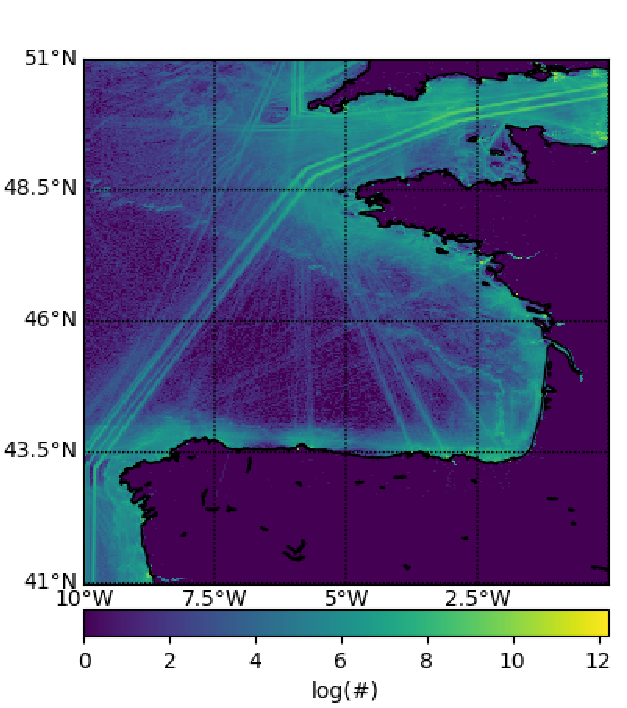
\includegraphics[width=0.8\linewidth]{CELTICcrop.pdf} 
    \caption{Logarithm applied} 
    \label{fig7:a} 
    \vspace{4ex}
  \end{subfigure}%% 
  \begin{subfigure}[b]{0.5\linewidth}
    \centering
    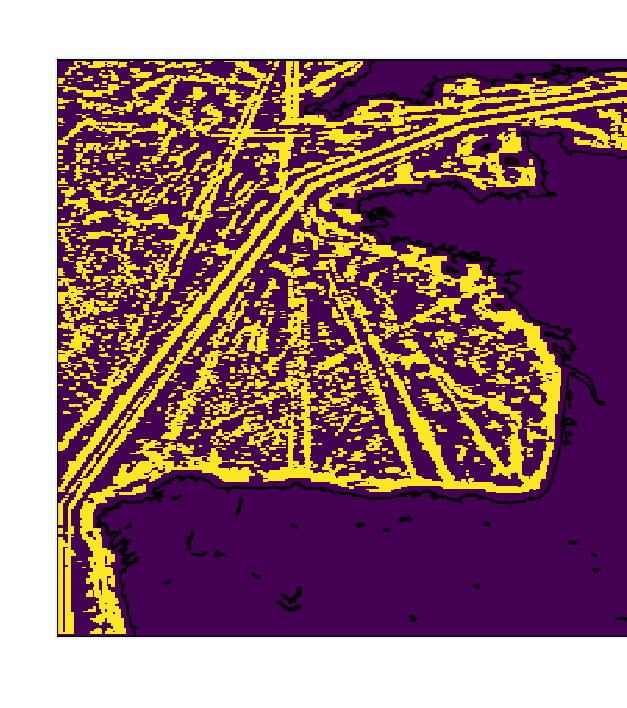
\includegraphics[width=0.8\textwidth]{CELTICopened-crop.pdf} 
    \caption{Binary segmented image} 
    \label{fig7:b} 
    \vspace{4ex}
  \end{subfigure} 
  \begin{subfigure}[b]{0.5\linewidth}
    \centering
    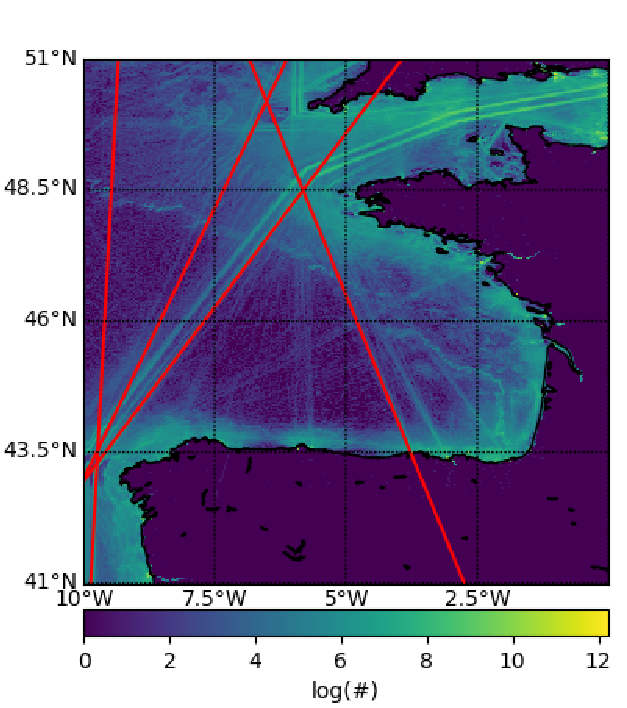
\includegraphics[width=0.8\textwidth]{CELTIClines-crop.pdf} 
    \caption{Hough Transform} 
    \label{fig7:c} 
  \end{subfigure}%%
  \begin{subfigure}[b]{0.5\linewidth}
    \centering
    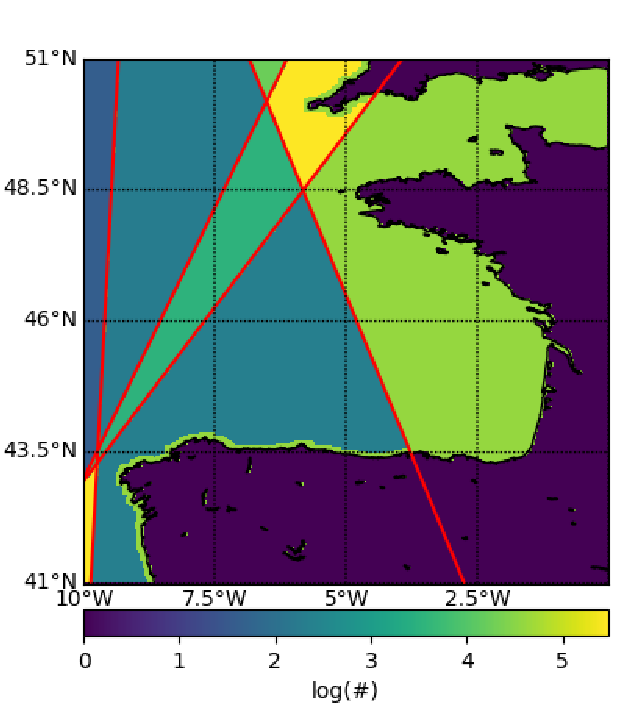
\includegraphics[width=0.8\textwidth]{CELTICsegmented-crop.pdf} 
    \caption{Segmented image} 
    \label{fig7:d} 
  \end{subfigure} 
  \caption{A heat-map of AIS ship positions within the Celtic sea, the Channel and the Bay of Biscay (France) [Longitude between $-10^{\circ}$ and $0^{\circ}$ and Latitude between $45^{\circ}$ and $51^{\circ}$]. The above subfigures were generated by applying the segmentation algorithm depicted in Algorithm 1 to an existing heat-map of the region. The top left image was optained after the logarithm of the original heat-map was taken (element-wise). The top right image 
  was obtained by applying binary thresholding and morphological opening to a filtered variant of the top left heat map. The right bottom heat-map depicts the lines we were able to extract 
  from the top right image using the Hough Transform. The bottom right image contains the final segmented heat map. Notice that the coastline is segmented separately.}
  \label{fig7} 
\end{figure}

\end{document}
